\newpage
\section{Grundlagen}

\subsection{Verwendete Hardware}
\subsubsection{Controller}
Diese Arbeit verwendet das von Atmel entwickelte Board "\board" \cite{src_SAMR}. Das Board besitzt neben einem ARM Cortex-M0+ Prozessor noch einen energiesparenden ISM-Bandsender-Empfänger auf einem Chip. Dieser Sender nutzt die Frequenz \SI{2,4}{\giga \hertz} zur Datenübertragung. Mit den vorhandenen GPIOs kann das Board verschiedene Sensoren und Aktoren ansteuern. Damit wird das \board \platz zu einem universell einsetzbaren Board für die drahtlose Kommunikation, speziell geeignet für den Embedded Bereich. Die folgende Abbildung \ref{img:samr21} zeigt das \board Board von der Vorderseite.
\begin{figure}[!ht]
	\centering
	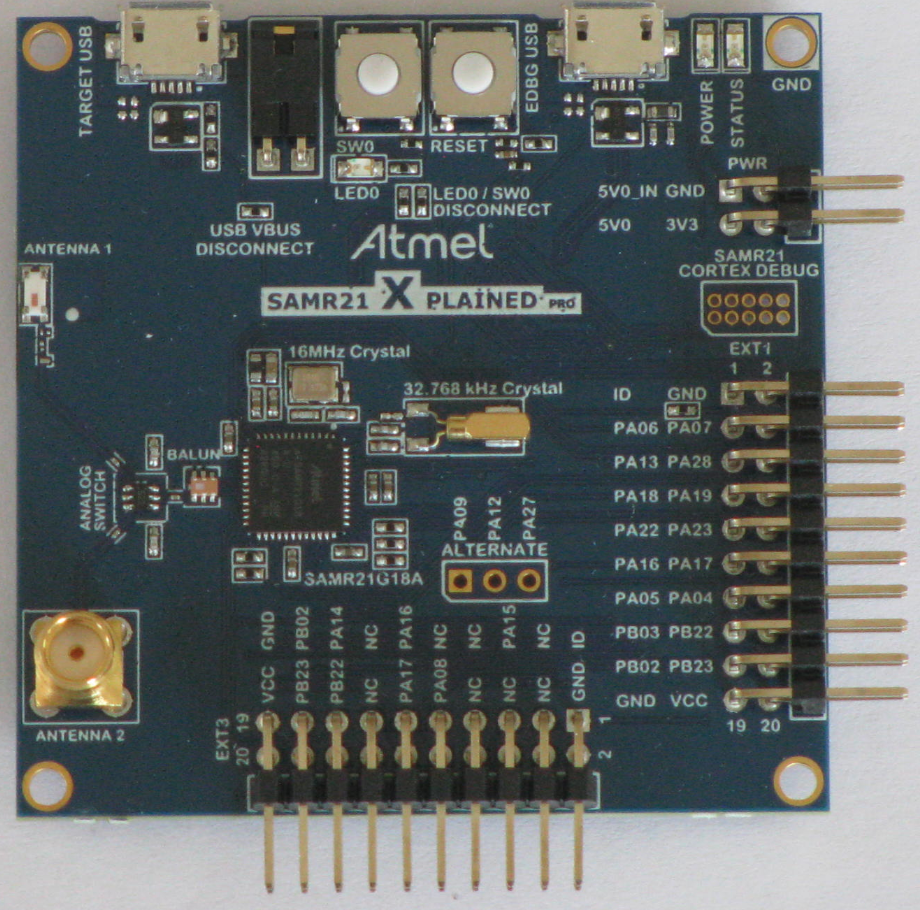
\includegraphics[width=0.6\textwidth]{images/samr21.png}
	\caption{Vorderseite des \board Board}
	\label{img:samr21}
\end{figure}

\subsubsection{Sensoren}
Für die Laufzeitmessung können verschiedene Sensoren verwendet werden. Im Folgenden wird ein Vergleich zwischen dem Ultraschallsensor \ultraschall \platz und dem \microphone \platz Sensor vorgenommen. Ein Vergleich ist notwendig, weil beide Sensoren in der Entwicklung zum Einsatz kamen, aber nur einer die nötige Performance für die Positionsbestimmung leistet.

%als alternative subsubsubsection
\paragraph{Ultraschallsensor}\mbox{}\\
Für die Positionsbestimmung ist der Ultraschallsensor \ultraschall \platz (Abbildung \ref{img:ultraschallsensor}) zum Einsatz gekommen \cite{src_HC_SR04}. Aus den folgenden Gründen wurde sich für den \ultraschall \platz Sensor entschieden: weite Verbreitung im Arduino/Raspberry-Pi-Bereich, kompakte Bauweise, geringe Anschaffungskosten und einfache Ansteuerung.

\begin{figure}%[!ht]
\centering
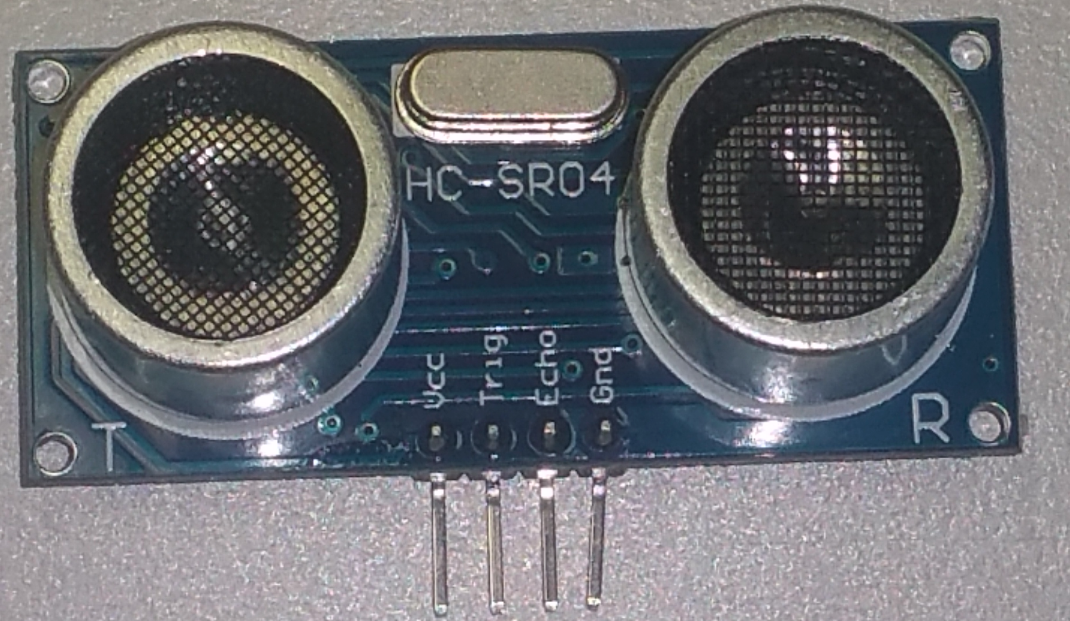
\includegraphics[width=0.6\textwidth]{images/ultraschallsensor.png}
\caption{Vorderseite des \ultraschall \platz Sensors}
\label{img:ultraschallsensor}
\end{figure}

In der Regel werden Ultraschallsensoren verwendet, um Distanzen zu einem Gegenstand zu ermitteln. Dabei wird ein Ultraschallsignal ausgesendet, welches von dem Gegenstand zurück reflektiert und wieder empfangen wird. Über die Zeitdifferenz zwischen Aussenden und Empfangen des Ultraschallsignals kann die Distanz berechnet werden. Aus der Abbildung \ref{img:ultraschall_prinzip} wird das Prinzip deutlich. Der \ultraschall \platz hat eine Reichweite von \SI{3}{\centi \metre} bis \SI{400}{\centi \metre}. Der Vorteil von diesem Ultraschallsensor ist, dass er ohne weitere Sensoren auskommt. Allerdings weißt er auch einige Nachteile auf, weswegen er von einem leistungsfähigeren Schallmikrofon (\microphone) abgelöst worden ist. Ultraschallsensoren funktionieren nur, wenn sie direkten Sichtkontakt zum Objekt haben. Dies ist nicht immer gegeben. Des Weiteren können nur Objekte, die in dem Sendekegel des Ultraschallsensors liegen, detektiert werden. Der Sendekegel für den \ultraschall \platz liegt bei \SI{15}{\degreeCelsius}, was eine Positionsbestimmung stark beeinträchtigt. Aufgrund der oben genannten Nachteile wurde sich in der Endanwendung gegen diesen Sensor entschieden.

\begin{figure}[H]
        \centering
        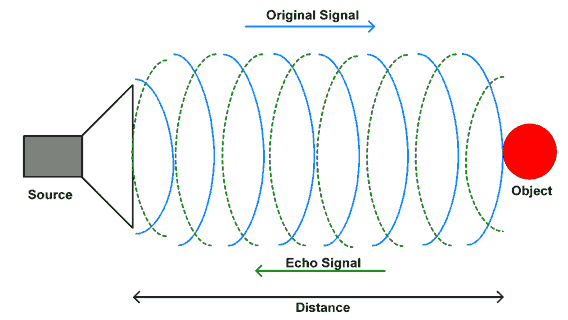
\includegraphics[width=0.6\textwidth]{images/ultraschall_prinzip.png}
        \caption{Funktionsweise von Ultraschallsensoren}
        \source{http://ceg.annauniv.edu/internship/2018/intern\_one/ECE/ECE5.pdf}
        \label{img:ultraschall_prinzip}
\end{figure}

\paragraph{Sound Detector}\mbox{}\\

\begin{figure}[H]
        \centering
        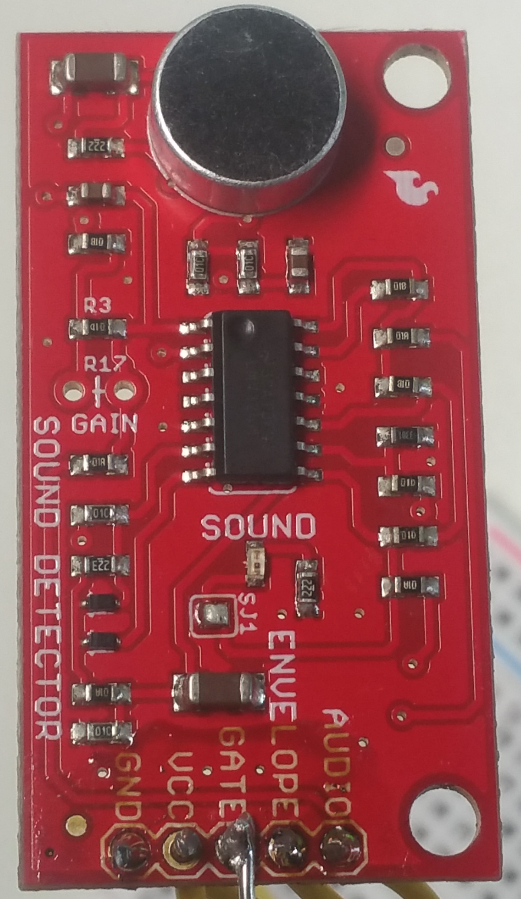
\includegraphics[width=0.4\textwidth]{images/sounddetector.png}
        \caption{Sparkfun Sound Detector}
        \label{img:sound}
\end{figure}

Abbildung \ref{img:sound} zeigt den \microphone. Der Sensor kann hörbaren Schall detektieren und darüber hinaus die Empfindlichkeit durch das Einlöten eines Widerstandes erhöhen oder verringern. Der Vorteil gegenüber dem Ultraschallsensor liegt darin, dass der Schall sich kugelförmig ausbreiten kann. Somit muss der Sensor nicht auf eine Richtung ausgerichtet werden. Allerdings stellen Hindernisse für einen hörbaren Schall ein Problem dar. Deswegen sollten keine oder nur wenige Hindernisse auf der Ebene vorhanden sein. Die Reichweite kann über eine Amplitudenveränderung des Tongebers variiert werden. Für die Ansteuerung des \microphone \platz gibt es die Möglichkeit, den digitalen Ausgang \si{GATE} zu verwenden. Neben diesem Ausgang gibt es noch weitere Ausgänge, allerdings werden diese nicht verwendet \cite{src_SOUND_DETECTOR}. Sobald ein Signal die eingestellte Schallschwelle überschreitet, wird der \si{GATE}-Ausgang des Sound Detectors auf \si{HIGH} gesetzt. Wird die Schallschwelle unterschritten, fällt der \si{GATE}-Ausgang zurück auf \si{LOW}. Abbildung \ref{img:gate_ausgang} zeigt ein Überschreiten des Schallpegels (Pegelwechsel).
 
\begin{figure}[H]
        \centering
        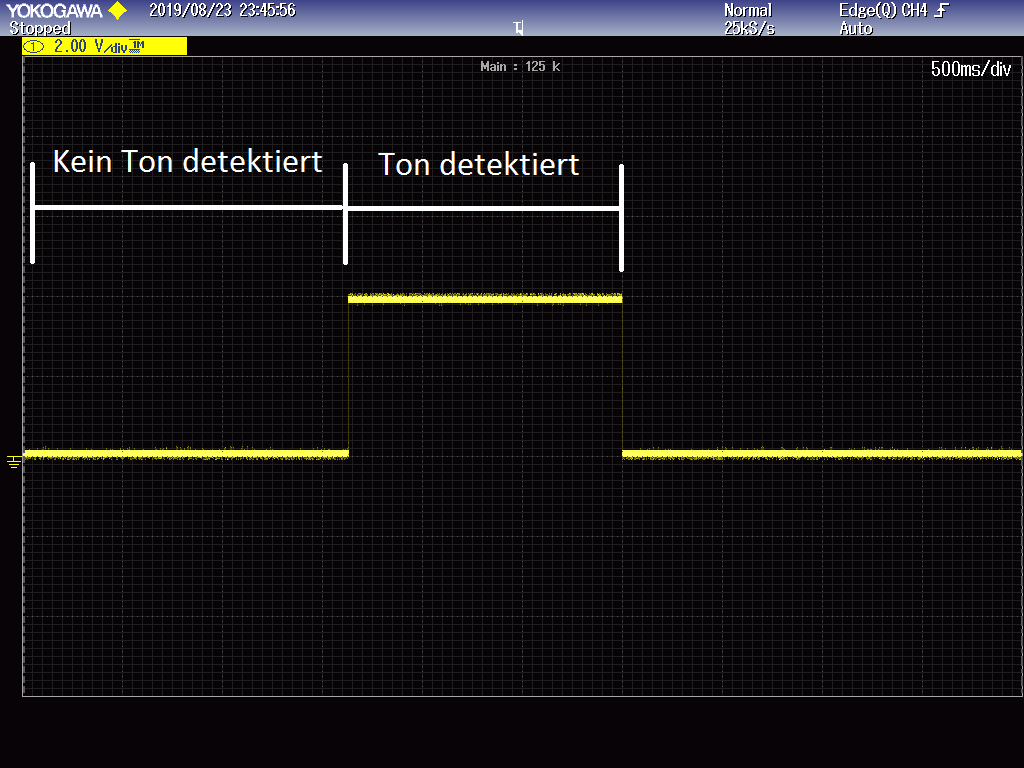
\includegraphics[width=0.95\textwidth]{images/gate_ausgang.png}
        \caption{Pegelwechsel des \si{GATE}--Ausgang}
        \label{img:gate_ausgang}
\end{figure}

\paragraph{\funkempfaenger}\mbox{}\\
Dieser Funksender sendet auf der \SI{433}{\mega \hertz} Frequenz \cite{src_433_FUNKSENDER}. Er ist im Arduino-Umfeld weit verbreitet und aufgrund seiner schlichten Ansteuerung einfach zu bedienen. Der Funksender besitzt keine Fehlerkorrektur für verlorene Nachrichten, sowie keine Signalkodierung. Deswegen eignet er sich gut für geringe Bandbreiten. Die Arbeit verwendet diesen Sensor, um ein Startsignal zu senden. Im Verlauf der Anwendung hat sich allerdings gezeigt, dass diese Variante nicht fehlerfrei funktionierte. Abbildung \ref{img:433_sender_empf} zeigt ein Foto des \funkempfaenger s.

\begin{figure}[H]
	\hspace*{-2cm}
    \subfigure[Funksender]
    {
    	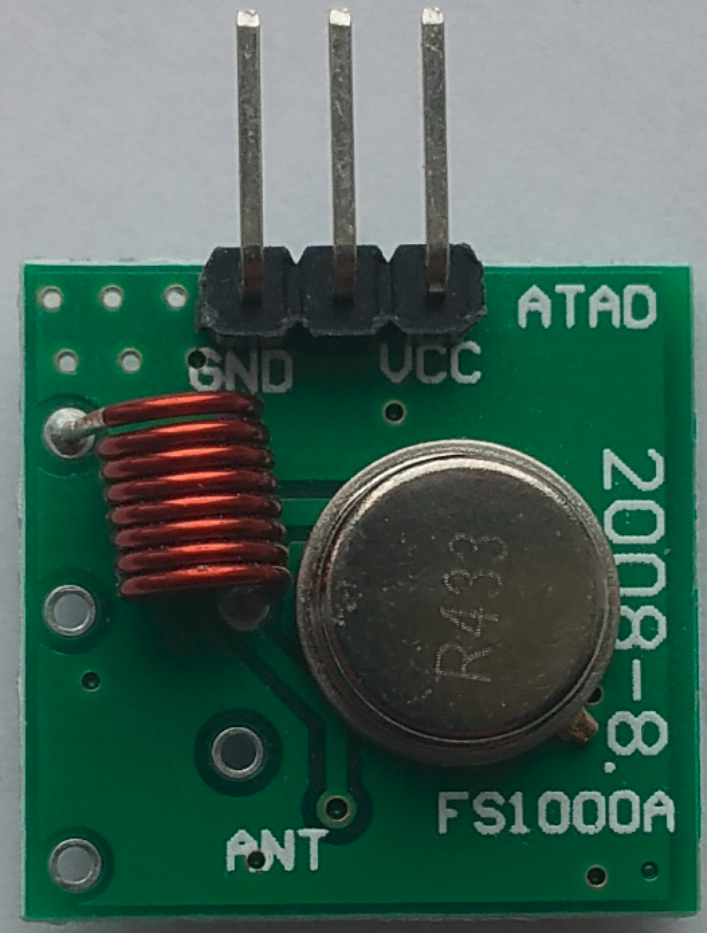
\includegraphics[width=0.5\textwidth]{images/sender.png}
    }	
    \subfigure[Empfänger]
    {
    	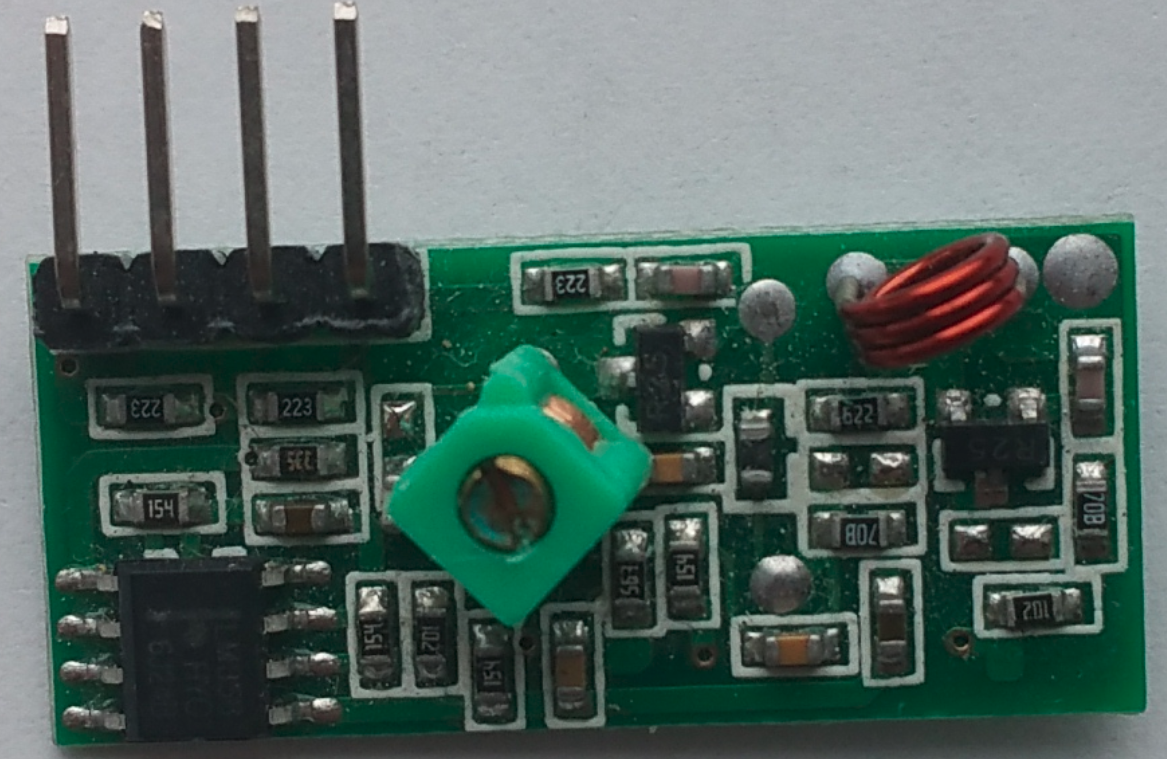
\includegraphics[width=0.7\textwidth]{images/empf.png}
    }
	\caption{\funkempfaenger}
	\label{img:433_sender_empf}
\end{figure}

Es folgt eine Auflistung der Anschlüsse des Funksenders (a) (von links aus gezählt):

\begin{description}[style=multiline,leftmargin=3cm]
\item [GND] 	Masse
\item [DATA]	Payload
\item [VCC]		Versorgungsspannung
\end{description}

Der Empfänger (b) besitzt vier Anschlüsse. Diese sind wie folgt (von links aus gezählt):

\begin{description}[style=multiline,leftmargin=3cm]
\item [GND] 	Masse
\item [DATA]	Payload
\item [DATA]	Payload
\item [VCC]		Versorgungsspannung
\end{description}

Mit einem Pegelwechsel des Funksenders bei dem Anschluss \si{DATA} kann eine Nachricht übertragen werden. Der Empfänger gibt die empfangenen Daten über die \si{DATA}-Anschlüsse wieder aus. Mithilfe eines Schmitt-Triggers kann dieses Signal geglättet werden.

\paragraph{Lautsprecher}\mbox{}\\
Als Tongeber wird ein handelsüblicher aktiver Lautsprecher verwendet \cite{src_LAUTSPRECHER}. Im Vergleich zu passiven Lautsprechern muss die Frequenz nicht selbst erzeugt werden. Mit dem Anlegen der Betriebsspannung wird die Membran in Schwingung versetzt. Die Lautstärke wird über die Betriebsspannung reguliert. Da der Lautsprecher mit \SI{24}{\volt} betrieben wird, benötigt man eine externe Schaltung. Diese besteht aus einem n-dotierten Mosfets und dem Lautsprecher. Abbildung \ref{img:schaltung} zeigt die Schaltung. Wenn an dem \si{GATE}-Eingang des Mosfet eine Spannung von \si{2} bis \SI{4}{\volt} anliegt, schaltet der Mosfet durch, und der Lautsprecher wird mit Strom versorgt.

\begin{figure}[H]
        \centering
		\hspace*{-1.5cm}
        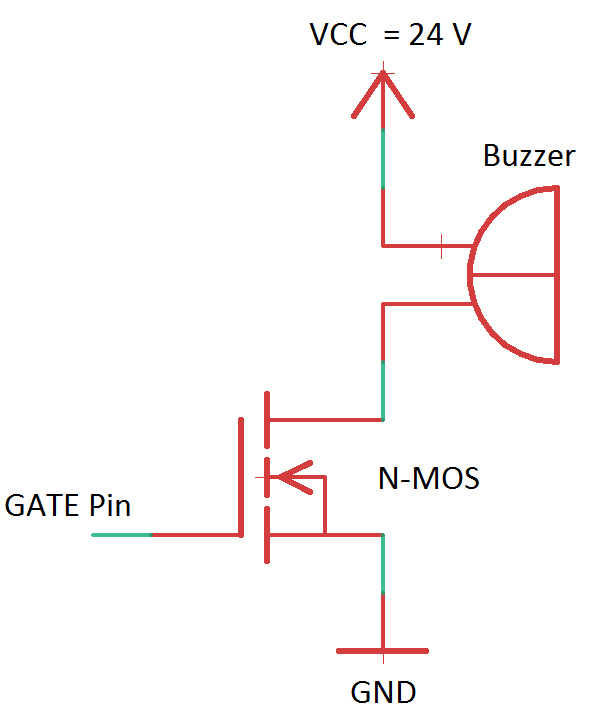
\includegraphics[width=0.65\textwidth]{images/schaltung.png}
        \caption{Ansteuerung des Lautsprechers}
        \label{img:schaltung}
\end{figure}


\subsection{Verwendete Software}
\subsubsection{RIOT OS}
Um das \board \platz in Betrieb nehmen zu können, kommt das echtzeitfähige Betriebssystem RIOT zum Einsatz. RIOT steht für: "The friendly Operating System for the Internet of Things" und wurde von der Freien Universität Berlin, der INRIA (Institut National de Recherche en Informatique et en Automatique), Le Chesnay, Frankreich und der Hochschule für Angewandte Wissenschaften, Hamburg, entwickelt. Es entstand aus dem "FeuerWhere" Projekt, bei dem Feuerwehrleute im Einsatz überwacht werden sollten. 2010 kam es zu einer Abspaltung des Projekts -- dies war die Geburtsstunde von RIOT. RIOT ist ein Betriebssystem für "Internet of Things"- Anwendungen. Es hat den Fokus auf drahtlose Sensornetzwerke gelegt. Protokolle wie 6LoWPAN, RPL, UDP und TCP wurden mit der Zeit implementiert. Des Weiteren unterstützt RIOT echtes Multithreading. Vergleicht man RIOT mit anderen Embedded-Betriebssystemen, erkennt man, dass RIOT die steigenden Anforderungen an Embedded-Betriebssystemen unterstützt. Weiterhin ist RIOT mit dem verwendeten Board \board \platz kompatibel, weshalb es sich perfekt als Betriebssystem für diese Arbeit eignet \cite{src_RIOT}. Abbildung \ref{img:vergleich} vergleicht RIOT mit drei anderen Betriebssystemen:

\begin{figure}[H]
        \centering
		\hspace*{-1.5cm}
        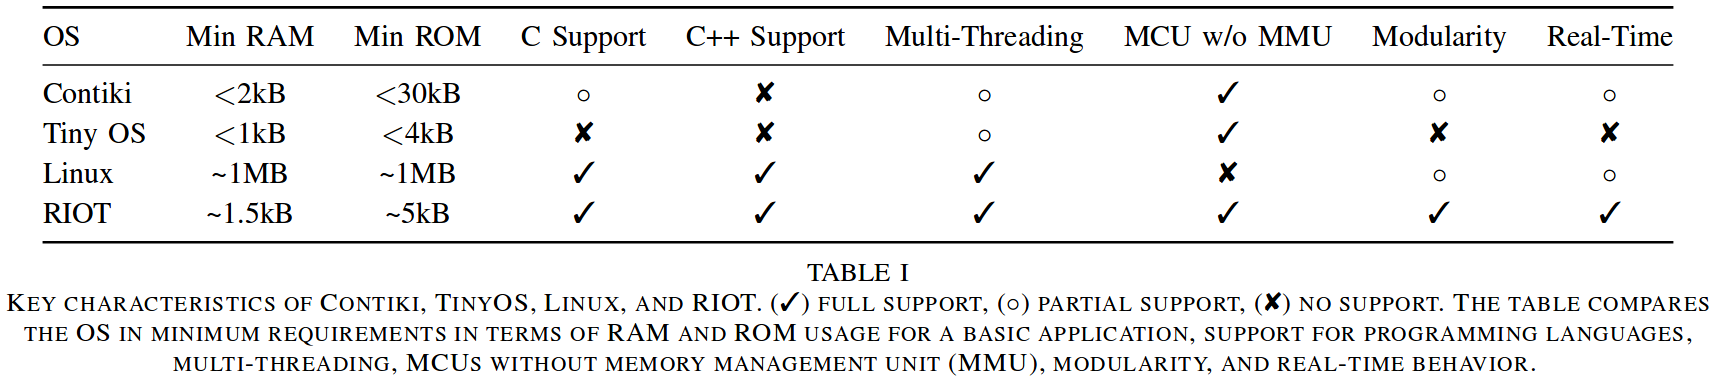
\includegraphics[width=1.2\textwidth]{images/vergleich.png}
        \caption{Vergleich von RIOT mit drei anderen Betriebssystemen}
        \source{https://www.riot-os.org/docs/riot-infocom2013-abstract.pdf}
        \label{img:vergleich}
\end{figure}

\subsection{Time Difference of Arrival -- TDOA}
Das TDOA ist ein Verfahren zur Laufzeitmessung, welches den Laufzeitunterschied eines Zeitstempels misst. Damit können Endgeräte über mindestens drei Basisstationen geortet werden. Für die Laufzeitmessung kann jede Art von Signal verwendet werden \cite{src_TDOA}.

\subsection{User Datagram Protocol -- UDP}
UDP ist ein Netzwerkprotokoll, welches im OSI-Modell in Schicht vier zu finden ist. UDP ist 1977 für die Sprachübertragung in Rechnernetzwerken entwickelt worden. Es ist gegenüber anderen Netzwerkprotokollen einfach aufgebaut. Es arbeitet verbindungslos, d.h. der Sender bekommt keine automatische Meldung, ob das gesendete Paket angekommen ist. Ein weiteres Netzwerkprotokoll zur Datenübertragung ist TCP. TCP steht für "Transmission Control Protocol" und es arbeitet im Gegensatz zu UDP verbindungsorientiert.
\\
UDP hat den Vorteil, dass vorher keine Verbindung mit dem Empfänger aufgebaut werden muss. Das ist besonders im IoT-Bereich wichtig, denn dort sind die Systeme meistens batteriebetrieben. Allerdings kann nicht ausgeschlossen werden, dass die Daten unverfälscht beim Empfänger ankommen.
\\
Ein UDP-Paket wird in ein Headerfeld und ein Datenfeld unterteilt. Die Größe des Headers sind immer 8 Byte. Es folgt eine Auflistung der Komponenten, aus denen das UDP-Paket besteht \cite{src_UDP}:
\\
\begin{description}[style=multiline,leftmargin=3cm]
\item [Quellport] Port des Quellrechners
\item [Zielport] Port des Zielrechners
\item [Länge] Gibt die Länge des Datensegmentes in Byte an
\item [Prüfsumme] Ein Wert, der aus dem Datensegment errechnet wird, um Manipulationen zu erkennen
\item [Daten] Nutzlast
\end{description}

\subsection{Netzwerk-Socket}
Ein Socket ist eine Schnittstelle, die vom Betriebssystem bereitgestellt wird. Es verbindet einen Kommunikationsendpunkt mit dem Betriebssystem. Über ein Socket kann ein Programm, welches eine Datei ist, auf den Kommunikationsendpunkt zugreifen. Wenn Netzwerkdaten empfangen werden, liegen diese zur Abholung im Socket bereit.
%Das vielleicht raus -> Nochmal nachhacken
%Sockets können bidirektional\footnote{Datenübertragung in beide Richtungen} betrieben werden. Sockets sind immer an einen Port gebunden.
UDP-Sockets sind immer an einen Port gebunden. Dadurch weiß das Betriebssystem, welche Pakete zu welchem Socket gehören. Neben UDP-Sockets gibt es noch RAW-Sockets. RAW-Sockets erlauben den Zugriff auf das ganze Paket. Dort werden keine Daten vorher aus dem Paket gefiltert \cite{src_SOCKET}.

\subsection{Indoor/Outdoor Positionsbestimmung}
Indoor-Positionsbestimmungssysteme sind nicht so weit verbreitet wie Outdoor-Systeme. Für Outdoor-Positionsbestimmungen wird häufig das globale Navigationssatellitensystem GPS (Global Positioning System) verwendet. Es kann aber auch der Mobilfunk genutzt werden. Für die Positionsbestimmung im Indoorbereich existieren mehrere Verfahren. Dazu zählen Messungen des Einfallswinkels, Signalstärkemessungen oder Laufzeitmessungen. Da bereits entschieden worden ist, dass wir Schall für die Positionsbestimmung nehmen, wird das Verfahren der Laufzeitmessung verwendet. Dabei wird die Zeitdifferenz zwischen Sende- und Empfangszeit ermittelt, sodass man die Signallaufzeit erhält \cite{src_INDOOR_OUTDOOR_SYSTEME}. Zusammen mit der Ausbreitungsgeschwindigkeit von Schall (\SI{343,2}{\metre\per\second} bei \SI{20}{\degreeCelsius}), kann somit die Distanz über die folgende Formel \ref{eq:formel_laufzeitmessung} berechnet werden:
\begin{equation}
	Distanz \;[\si{\metre}] = (Empfangszeit - Sendezeit)\;[\si{\second}]\quad \cdot \quad Ausbreitungsgeschwindigkeit \;[\si{\metre\per\second}]
   \label{eq:formel_laufzeitmessung}
\end{equation}

\subsection{Zeitsynchronisation}
Für eine Laufzeitmessung ist es wichtig, dass Sender und Empfänger die gleiche Uhrzeit haben. Damit eine hohe Genauigkeit bei der Laufzeitmessung erreicht werden kann, muss der Zielknoten (Master) wissen, zu welchem Zeitpunkt der Accesspoint (Slave) den Schall aussendet. Ist dies nicht gewährleistet, müsste der Master raten. Damit dies nicht geschehen muss, ist es notwendig, dass beide Knoten die gleiche Zeitbasis haben. Für dieses Problem wird eine Zeitsynchronisation für drahtlose Netzwerke verwendet: das Precision Time Protocol (PTP). PTP ist für kleine hierarchielose Netzwerke entwickelt worden -- es gibt hierbei keine Hierarchien wie beim Network Time Protocol (NTP). Der Vorteil liegt darin, dass PTP nicht wie NTP mit jeder Hierarchie Genauigkeit verliert. Es spezialisiert sich auf kleine Netzwerke ohne Hierarchien. Um eine Genauigkeit im Nanosekundenbereich zu erreichen, muss die aktuelle Systemzeit kurz vor dem Absenden des Pakets hinzugefügt werden. Je geringer die Verzögerung zwischen dem Funktionsaufruf $getSystemTime()$ und dem Absenden des Pakets ist, desto genauer wird die Zeitsynchronisation. Abbildung \ref{img:ptp} zeigt, welchen Nachrichtenaustausch für die Zeitsynchronisation nötig ist. Der Master ist der Zeitgeber und der Slave synchronisiert seine Zeit. 
%Hier war Abbildung 9
Zuerst wird bei PTP die Laufzeitverzögerung ermittelt. Danach kommt es zur eigentlichen Synchronisation der Zeit. Für die Laufzeitverzögerung sendet zuerst der Master eine \si{SYNC}-Nachricht mit seinem Zeitstempel $t_{0}$ an den Slave. Aufgrund der Verarbeitungszeit, der Laufzeitverzögerung und der Zugriffszeit ist der Zeitstempel $t_{0}$ nicht präzise. Mit einer \si{FOLLOW\_UP}-Nachricht werden diese Probleme gemildert. Dabei enthält die \si{FOLLOW\_UP}-Nachricht den Zeitstempel $t_{0}$. Nach der \si{FOLLOW\_UP}-Nachricht weiß der Slave, wie groß die Laufzeitverzögerung ist. Die \si{FOLLOW\_UP}-Nachricht kann auch weggelassen werden, dafür muss allerdings der Master den Zeitstempel $t_{0}$ weit genug in der Zukunft bestimmen, sodass die Vorverarbeitung der \si{SYNC}-Nachricht abgeschlossen werden kann. Dann ist der Zeitpunkt des Aussenden der \si{SYNC}-Nachricht exakt gleich mit dem Zeitstempel $t_{0}$ -- diese Arbeit verwendet dies allerdings nicht, da die Genauigkeit der Systemzeit nicht exakt ist.
\\
Die \si{FOLLOW\_UP}-Nachricht wird mit dem Zeitstempel $t_{0}$ versehen und von dem Master ausgesendet. Somit ist nun die Laufzeitverzögerung bekannt.
Um nun den Offset zu bestimmen, sendet der Slave eine \si{DELAY\_REQ}-Nachricht -- ohne Inhalt. Dabei wird der Zeitstempel $t_{2}$ beim Absenden des Slave festgehalten. Der Master empfängt die \si{DELAY\_REQ}-Nachricht und speichert seinen Zeitstempel in der Variable $t_{3}$. Darauf wird mit einer \si{DELAY\_RESP}-Nachricht mit dem Inhalt des Zeitstempels $t_{3}$ geantwortet. Der Slave empfängt die Nachricht und speichert bei Empfang in $t_{4}$ seinen Zeitstempel. Nun kann mit den folgenden zwei Formeln (\ref{eq:formel_ptp}) die Zeitdifferenz berechnet werden. Dabei entspricht $\tau_{prop}$ der Laufzeitverzögerung und Omega (\si{\ohm}) ist der Zeitunterschied zwischen Master und Slave \cite{src_PTP}.

\begin{equation}\label{eq:formel_ptp}
\begin{split}
\tau_{prop} = \frac{t_{1} - t_{0} + t_{3} - t_{2}}{2}
\\
\Omega = t_{1} - t_{0} - \tau_{prop}
\end{split}
\end{equation}

\begin{figure}[H]
        \centering
%		\hspace*{-1.5cm}
        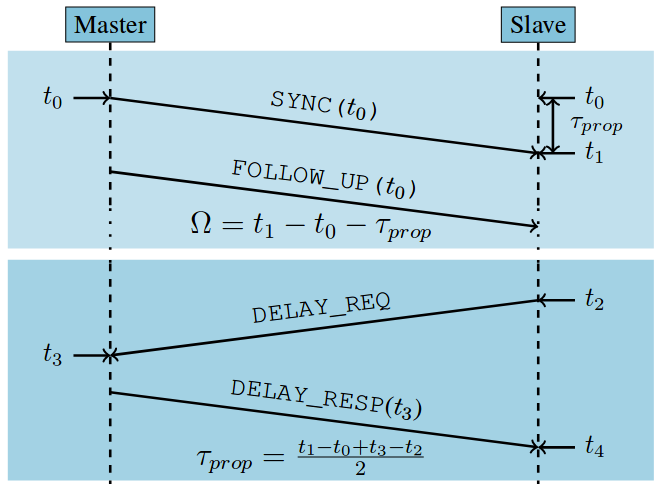
\includegraphics[width=0.9\textwidth]{images/ptp.png}
        \caption{Nachrichtenaustausch in PTP}
        \source{https://www.ibr.cs.tu-bs.de/oa/vonzengen\_ICIT2017.pdf}
        \label{img:ptp}
\end{figure}

\subsection{Mathematischer Hintergrund -- Positionsbestimmung}

Damit auf einer Ebene die Position bestimmt werden kann, muss der Master von mindestens drei Slaves die Distanz messen. Da sich der Schall auf einer Ebene kreisförmig ausbreitet, konzentriert sich das Problem auf den Schnittpunkt von nur drei Kreisen (Abbildung \ref{img:positionsbestimmung}). Des Weiteren müssen die Koordinaten der Slaves bekannt sein.
\begin{figure}[H]
\centering
% \hspace*{-1.5cm}
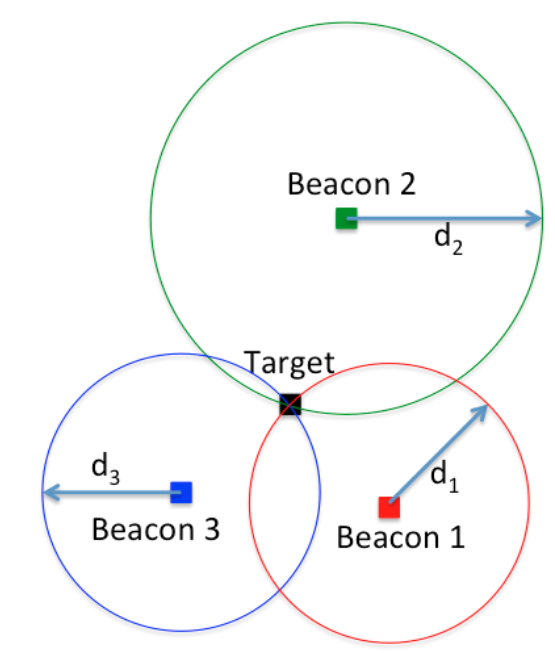
\includegraphics[width=0.5\textwidth]{images/positionsbestimmung.png}
\caption{Prinzip der Positionsbestimmung}
\source{https://sites.tufts.edu/eeseniordesignhandbook/files/2017/05/FireBrick\_OKeefe\_F1.pdf}
\label{img:positionsbestimmung}
\end{figure}
Aufgrund von Schwankungen kann es vorkommen, dass es keinen gemeinsamen Schnittpunkt der drei Kreise gibt, wie Abbildung \ref{img:positionsbestimmung} vermittelt. Deswegen wird ein Bereich angegeben, wo sich der Master befinden muss. Je größer die Schwankungen bei der Distanzmessung sind, desto größer ist der Zielbereich \cite{src_MATH_TDOA}. Abbildung \ref{img:schwankungen} verdeutlicht das Problem. Dort befindet sich der Master zwischen den folgenden Punkten:

\begin{equation}
\begin{split}
A: \; (2,7671\;|\;3,3700) \\
B: \; (3,1775\;|\;2,5081) \\
C: \; (2,2727\;|\;1,4454)
\end{split}
\end{equation}

\begin{figure}[H]
\centering
% \hspace*{-2.7cm}
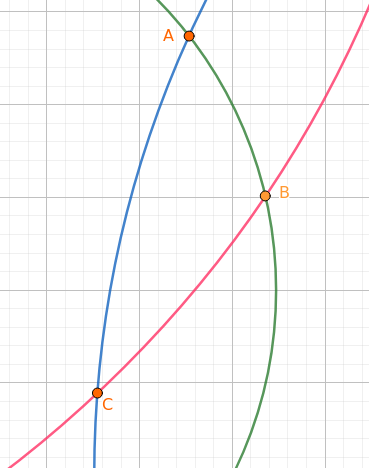
\includegraphics[width=0.7\textwidth]{images/positionsbestimmung_flaeche.png}
\caption{Bereich indem sich der Zielknoten befinden muss}
\label{img:schwankungen}
\end{figure}

Die Normalform für eine Kreisgleichung mit Mittelpunkt $(x_{0}|y_{0})$ und Radius $r$ lautet:
\begin{equation}
(x-x_{0})^{2}+(y-y_{0})^{2} = r^{2}
\end{equation}

Mit Hilfe der drei Kreise (A, B, C) (Abbildung \ref{img:positionsbestimmung}) kann nun der Schnittpunkt berechnet werden -- siehe folgendes Gleichungssystem \ref{eq:gleichungssystem}. Dabei entsprechen $x_{A}$, $y_{A}$ den Mittelpunkt von Kreis $A$ mit Radius $r_{A}$. Diese Notation wird auch auf Kreis $B$ und $C$ angewendet.

\begin{equation} \label{eq:gleichungssystem}
\begin{split}
\RM{1} \quad (x-x_{A})^{2}+(y-y_{A})^{2} &= r_{A}^{2} \\
\RM{2} \quad (x-x_{B})^{2}+(y-y_{B})^{2} &= r_{B}^{2} \\
\RM{3} \quad (x-x_{C})^{2}+(y-y_{C})^{2} &= r_{C}^{2}
\end{split}
\end{equation}

Um den Schnittpunkt zwischen allen drei Kreisen zu erhalten, muss das Gleichungssystem \ref{eq:gleichungssystem} nach $x$ und $y$ aufgelöst werden. Aufgrund von Schwankungen ist dies nicht immer möglich. Punkt \si{1} berechnet sich durch das Auflösen nach $x$ von $\RM{1}$ und $\RM{2}$ . Für Punkt \si{2} werden die Gleichungen $\RM{1}$ und $\RM{3}$ verwendet, für den dritten Punkt $\RM{2}$ und $\RM{3}$. Die Herleitung ist im Anhang (Seite \pageref{sec:abcdef}) aufgeführt.

